

\subsection{Problem Statement and Method Overview}
Existing dexterous grasp pose generation methods remain limited in their ability to model semantic information, particularly in scenarios requiring fine-grained control. This limitation restricts further improvements in the precision and adaptability of dexterous grasp strategies. Moreover, the scarcity of grasp datasets with rich, multi-dimensional semantic annotations continues to hinder progress in this research direction.

To address these challenges, we propose a semantic-sensitive dexterous grasp dataset generation method OmniDexDataGen that incorporates multiple levels of semantic information, from functional affordance, contact configuration, to grasp taxonomy,  as introduced in Sec.~\ref{sec:dataset_generation_grasp_taxonomy_aware}. Building upon this foundation, we develop a semantic reasoning pipeline based on large multimodal models OmniDexReasoner to enhance the understanding of object-grasp relationships and grasp type, as shown in Sec.~\ref{sec:dexterous_grasping_semantic_label_generation}. We further introduce a 3D vision-language model for semantically guided dexterous grasp pose generation, named OmniDexGraspNet, as detailed in Sec.~\ref{sec:3d_vision_language_dexterous_grasp_generation}. 


\subsection{Functional Affordance-Aware and Contact-Sensitive Dexterous Grasp Dataset Generation Enriched by Grasp Taxonomic Diversity}
\label{sec:dataset_generation_grasp_taxonomy_aware}
We propose a dexterous grasp data generation method that is sensitive to both functional affordance and grasp taxonomy, as shown in Fig.~\ref{fig:grasp_generation_pipeline}. This method integrates the functional regions of the object, the contact configurations, and the opposition types associated with various grasp taxonomies. By leveraging an optimization-based strategy, our approach generates high-quality grasp samples with enhanced functional diversity, contact semantic diversity, and grasp taxonomy diversity. The proposed grasp generation pipeline consists of following key parts: Grasp-type-aware configuration sampling, functional affordance-aware contact point sampling (AC-Sampler), grasp taxonomy-aware DFC grasp pose sampling (Tax-DFCSampler), and grasp optimization method.

In the grasp-type-aware configuration sampling stage, representative grasp configurations are automatically sampled according to the dexterous hand grasp taxonomy. In the affordance- and grasp-type-guided pose sampling method, initial grasp poses are sampled within object affordance regions based on task semantics and grasp-type constraints, including opposition type and corresponding contact configuration. Finally, optimization method refines the sampled grasp poses using functionality- and taxonomy-aware hand–object interaction loss and validates them through physical evaluation to ensure reliable data generation.

\subsubsection{Grasp Taxonomy-Aware Configuration Sampling}

Originating from grasp taxonomy analysis~\cite{feix2015grasp}, different grasp types are typically characterized by specific opposition types, force directions, involved fingers in hand–object contact, contacting links of each finger, and the spatial distribution of contact regions. 
We define a structured representation of a grasp configuration, which includes: the set of activated fingers $S_f$ participating in the grasp, the specific links $S_l$ of each finger that are involved in contact, the contact regions $S_c$ associated with each link and the force direction $v$ and grasp central point $c$.

The goal of grasp configuration sampling is to generate an appropriate grasp configuration $G = \{S_f, S_l, S_c, v, c\}$ given a specified grasp type $t_g$. 

Formally, the grasp configuration sampling process is defined as:
\begin{equation}
    G = f_{\rm config}(t_g)
\end{equation}
where $G$ denotes the generated grasp configuration, and $f_{\rm config}$ is the grasp configuration sampling method conditioned on the specified grasp type.



\subsubsection{Functional Affordance-Aware and Grasp Type-Aware Differential Force-Closure Grasp Sampling}


Building on our proposed grasp configuration modeling, we further introduce a Differential Force Closure (DFC)-based grasp pose sampling method (Tax-DFCSampler) that is sensitive to both functional affordance and grasp type. This method is designed to generate initial grasp pose candidates, enhancing the semantic diversity and physical plausibility of the resulting grasp set. The sampling pipeline is detailed in Alg.~\ref{alg:dfc_gps}. 

The objective of Tax-DFCSampler is to, given a specific grasp configuration, incorporate object-level functional affordance information to generate a set of physically plausible contact points and estimate their corresponding initial grasp poses. The process can be formally defined as:
\begin{equation}
    \{G_{\rm init}, C_{\rm init}\} = f_{\rm Tax-DFCSampler}(M_{\rm obj}, G)
\end{equation}
where, $G_{\rm init}$ is the initial grasp pose. $C_{\rm init}$ denotes the corresponding set of contact points. $M_{\rm obj}$ is the object mesh annotated with an affordance map. $G$ is the grasp configuration and $f_{\rm Tax-DFCSampler}$ is the grasp sampling function.

To enhance sensitivity to functional affordance, functional affordance contact point sampling method (AC-Sampler) first samples two primary contact points $C$  from the affordance map of the object surface. These candidate contacts are then validated using a DFC estimator $f_{\rm DFC}$~\cite{liu2021synthesizing} to ensure that they meet force-closure constraints. 
\begin{equation}
\begin{gathered}
f_{\rm DFC}=\|G c\|^2 \\
G=\left[\begin{array}{ccc}
I_3 & \cdots & I_3 \\
{\left[\psi_1\right]_{\times}} & \cdots & {\left[\psi_n\right]_{\times}}
\end{array}\right] \\
{\left[\psi_k\right]_{\times}=\left[\begin{array}{ccc}
0 & -\psi_k^{(z)} & \psi_k^{(y)} \\
\psi_k^{(z)} & 0 & -\psi_k^{(x)} \\
-\psi_k^{(y)} & \psi_k^{(x)} & 0
\end{array}\right]}
\end{gathered}
\end{equation}
where, $\Psi=\{\psi_1, \cdots,\psi_n\}$ denotes the set of contact point candidates. term $c \in \mathbb{R}^{n \times 3}$ represents the normals of object surface at the contact points in~$\Psi$, and $n$ indicates the number of contact points. 
Specifically, an oversampling strategy is employed, allowing the DFC estimator to filter out physically infeasible candidates and retain a batch-sized set of valid contact points. The mid-point between $C_m$ is selected as the grasp central point for further initial hand pose alignment, and random permutations are added to increase diversity in the resulting grasp poses.


Next, finger joint poses are initialized based on sampled the hand configuration according and the grasp type. 
By default, the initial pose is defined such that the index finger and thumb are positioned in opposition, enabling a neutral pre-grasp configuration commonly used for precision or pad opposition grasps. However, for grasp types that involve side contact regions, the initial hand open pose is specifically adapted to place the thumb in a side opposition configuration. Then, to generate contact points for all activated fingers, all fingertip contact points of all activated fingers are projected along the contact force direction onto the object surface to obtain a full set of candidate contact points. To prevent overfitting to a single structure, the non-activated fingers are randomly perturbed. Following this, we perform parallel hand-object collision checking using the kinematic skeleton of the dexterous hand. Specifically, the generated grasp candidates are split into multiple chunks for efficient parallel evaluation. 
For each pose, the number of collisions between hand links and the object is computed. Only those candidates with a collision count below a predefined threshold are retained as valid initial grasp poses $G_{\rm init}$.



\begin{algorithm}[t]
\caption{Functionality- and Grasp-Type-Aware Grasp Pose Sampling (AC-Sampler + Tax-DFCSampler)}
\label{alg:dfc_gps}
\begin{algorithmic}[1]
\REQUIRE $M_{\text{obj}}$: Object mesh with functional affordance map \\
         $G$: Grasp configuration from taxonomy \\
         $f_{\text{DFC}}$: Differential Force Closure estimator \\
         $N$: Number of required grasp candidates \\
         $\tau$: Collision threshold
\ENSURE $G_{\text{init}}$: Set of valid initial grasp poses

\STATE $C_{\text{valid}} \leftarrow \emptyset$
\WHILE{$|C_{\text{valid}}| < N$}
    \STATE $C_m \leftarrow$ SamplePrimaryContacts($M_{\text{obj}}$, $G$)
    \IF{$f_{\text{DFC}}(C_m)$ is valid}
        \STATE $C_{\text{valid}} \leftarrow C_{\text{valid}} \cup \{C_m\}$
    \ENDIF
\ENDWHILE

\STATE $G_{\text{init}} \leftarrow \emptyset$
\FOR{each $C$ in $C_{\text{valid}}$}
    \STATE $C_m' \leftarrow$ RandomSwap($C_m$)
    \STATE $d \leftarrow$ GetForceDirection($G$)
    \STATE $F_{\text{act}} \leftarrow$ GetActivatedFingers($G$, $d$)
    \STATE $p_{\text{center}} \leftarrow$ EstimateGraspCenter($C_m'$, $d$)
    \STATE $G_{\text{pose}} \leftarrow$ ConstructHandPose($p_{\text{center}}$, $d$, $G$, addNoise= True)
    \STATE RandomizeIdleFingers($G_{\text{pose}}$)
    \STATE $n_{\text{col}} \leftarrow$ CheckCollision($G_{\text{pose}}$, $M_{\text{obj}}$)
    \IF{$n_{\text{col}} < \tau$}
        \STATE $G_{\text{init}} \leftarrow G_{\text{init}} \cup \{(G_{\text{pose}}, C_m')\}$
    \ENDIF
\ENDFOR
\RETURN $G_{\text{init}}$
\end{algorithmic}
\end{algorithm}



\subsubsection{Grasp Optimization and Simulation Validation}

After constructing the grasp configuration that incorporates functional affordance, grasp taxonomy, and contact sensitivity, and obtaining the initial grasp pose through DFC-based sampling, we further refine the candidate poses via an optimization procedure. During optimization, only the activated fingers and wrist pose are updated, while the non-activated fingers remain fixed to their original configuration.
The overall objective function comprises the following three key components: Semantic hand-object interaction loss, Differential Force Closure (DFC) estimation loss and Penetration and joint-limit regularization. 

The construction of the loss function proceeds as follows. 
For each activated finger, we randomly sample contact points from its designated contact region as specified by the grasp configuration. 
Corresponding target contact points are sampled from the object surface. 
The contact alignment is then optimized by computing the Signed Distance Function (SDF) between the hand mesh and object surface, minimizing interpenetration while encouraging semantically valid contact. 
The DFC estimator is employed as an additional optimization objective to promote high-quality, force-closure grasps. 
During the entire optimization process, joint angle updates are constrained by anatomical joint limits, ensuring biomechanically feasible and physically plausible hand postures.

After optimization, each refined grasp candidate is validated within a physics simulation environment. Specifically, we adopt a joint impedance control strategy to enable compliant yet stable dexterous grasping, simulating realistic contact forces and evaluating the stability of the grasp during execution. 
For each joint $i$, the control torque $\tau_{i}$ is computed as:
  \begin{equation}
\tau_i=k_i\left(q_i^{\text {target}}-q_i\right)-d_i \dot{q}_i+g_i
\end{equation}
where, $\tau_{i}$ denotes the torque applied to joint $i$, $q_i$ is the current joint position, $q_i^{\text {target}}$ represents target joint position, $\dot{q}_i$ denotes joint velocity, $k_i$, $d_i$ and $g_i$ are the stiffness, damping coefficients, and external compensation terms, respectively,
Only those grasp poses that successfully complete the simulated grasp—without slippage or failure—are retained in the final dataset. 


\begin{figure*}[htbp]
  \centering
  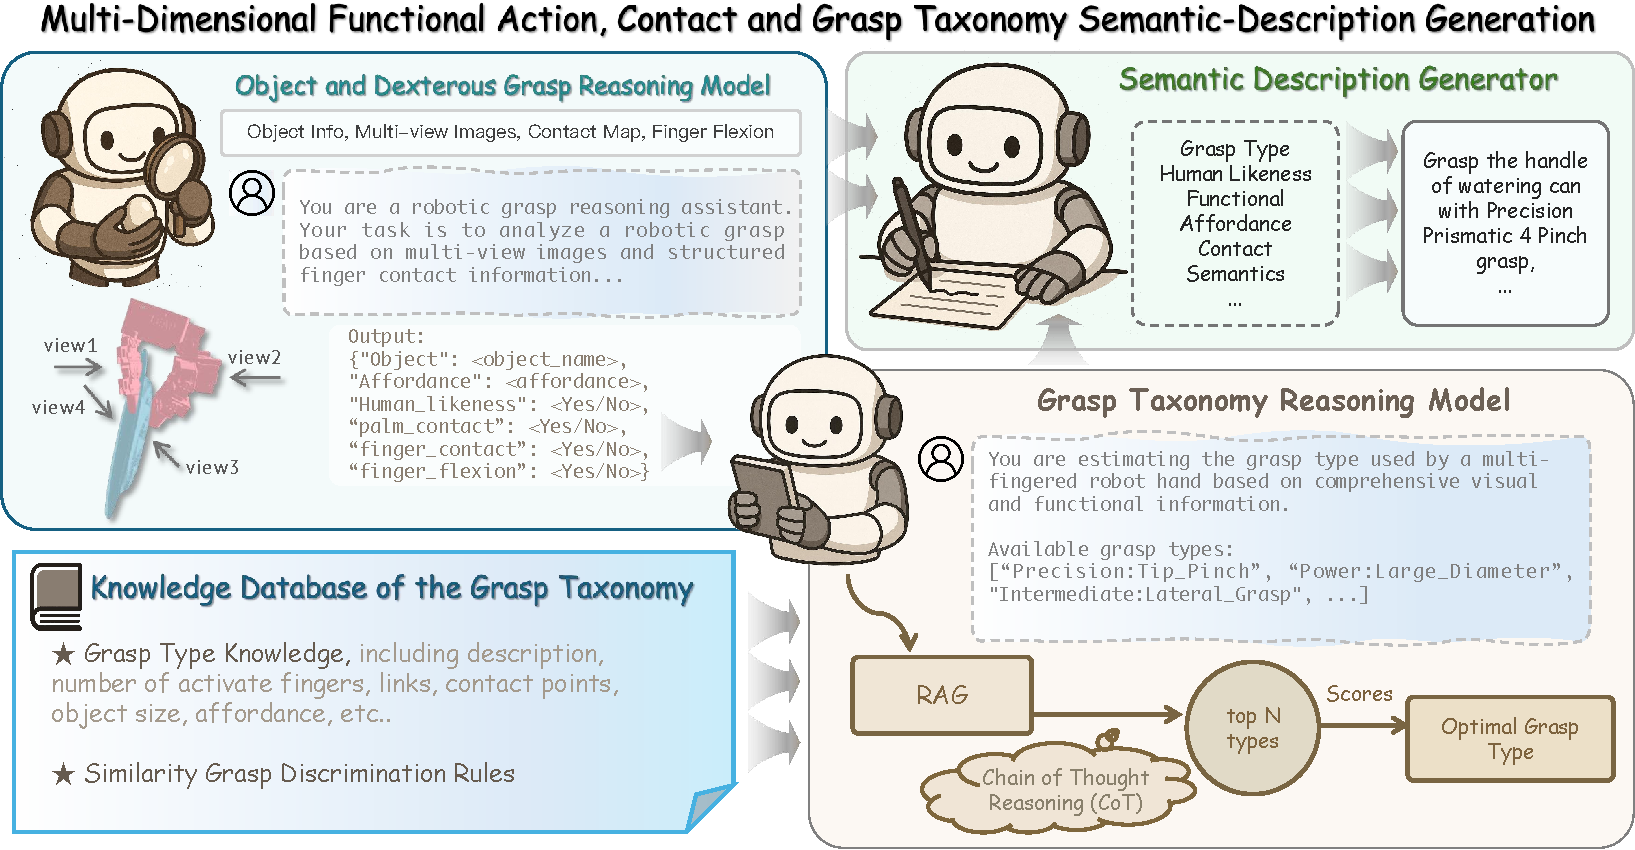
\includegraphics[width=1.0\linewidth]{pictures/fig_grasp_reasoning_agents.pdf}
  \caption{% 
  OmniDexReasoner: 
  LMM-Based dexterous grasping multi-dimensional semantic reasoning, including functional affordance, contact semantic information, finger configuration, grasp taxonomy and human-consistency.}
  \label{fig:semantic_understanding_lmm}
\end{figure*}

\subsection{LMM-Grounded Dexterous Grasping Multi-Dimensional Semantics Understanding Method}
\label{sec:dexterous_grasping_semantic_label_generation}


To enrich the generated grasp dataset with multi-dimensional semantic annotations, we propose OmniDexReasoner, a multimodal large model (LMM)-based semantic reasoning framework for dexterous grasping, which is sensitive to functional affordance, contact semantics, and grasp taxonomy, as shown in Fig.~\ref{fig:semantic_understanding_lmm}. By integrating multi-agent collaboration, Chain-of-Thought (CoT) reasoning, and Retrieval-Augmented Generation (RAG) strategies, the proposed framework addresses key gaps in current research on dexterous hand semantic understanding. 
Our semantic reasoning pipeline consists of three key modules: hand–object interaction understanding model, grasp taxonomy reasoning model and dexterous grasp multi-dimensional semantic generatior.  This framework enhances the expressiveness of semantic annotations in dexterous grasp datasets and provides high-quality semantic priors to support downstream multimodal models.

\subsubsection{Hand–Object Interaction Understanding Model}

To understand the interactive information between a robotic hand and an object, we propose a model for hand-object interaction understanding. This model leverages multimodal information, including object attributes, robotic hand configurations, hand-object contact data, and grasping scene images, to automatically predict the semantic relationships between the hand and the object. 
This process can be modeled in a probabilistic framework as:
\begin{equation}
    P(A|I)=P(A|H,O,C,V)
\end{equation}

where $A$ represents the semantic outputs of the model, and $I$ denotes the multimodal input. $H$ denotes information about the robotic hand, such as the types of available fingers, available finger links, joint configurations, and maximum graspable size. 
$O$ represents object-related information, including the object's name, affordance annotations. $C$ captures the contact information between the hand and the object, including the contact semantic map $M_c$ and corresponding grasp affordance estimation result $a^{*}$. 
$V$ refers to multi-view images of the grasping scene. Output $A$ contains of final functional affordance estimation classification result $a_{\rm sem}$, textual object descriptions, contact fingers and links, finger flexion configurations, palm contact status, and the contact semantic map.

To model the contact information, we compute the spatial distance between various links and fingers of the hand and surface points on the object, similar to~\cite{zhang2024contactdexnet}. This allows us to construct a Contact Semantic Map $M_c$, assigns semantic contact labels to the object surface points. The map is defined as:
\begin{equation}
M_c\left(p_i\right)=\left(l_j, f_k\right), \quad \text { if } \quad d\left(p_i, L_{j k}\right)<\delta
\end{equation}
where, $p_i \in \mathcal{P}$ denotes a surface point sampled from the object. $l_j$ denotes the 
j-th link. $f_k$ denotes the k-th finger. 
$L_{jk}$ is the 3D model of the j-th link on the k-th finger. $d(p_i, L_{jk})$ is the minimum Euclidean distance between $p_i$	
  and $L_{jk}$. $\delta$ is a contact threshold. Each contact point on the object surface is thus labeled with the corresponding hand link and finger involved in the contact.


Within the agent, the Contact Semantic Map is further analyzed to identify the involved fingers and links, and whether the palm is in contact with the object. Palm contact is a key indicator of grasp type, such as power grasp or precision grasp. However, the degree of force exerted by the palm requires further estimation using visual cues from the grasping scene.



To infer object affordances from hand-object interactions, we employ a voting-based functional grasp affordance classification method. This method integrates the Contact Semantic Map $M_c$ with an affordance label map $M_a$ defined over the object surface. For each contact point $p_i$, we count the associated affordance label and determine the most frequent one via voting:
 \begin{equation}
a^*=\arg \max _{a \in \mathcal{A}} \sum_{p_i \in \mathcal{P}} \mathbb{I}\left[M_c\left(p_i\right) \neq \emptyset\right] \cdot \mathbb{I}\left[M_a\left(p_i\right)=a\right]
\end{equation}
where, $a^*$ is the predicted functional affordance. $\mathcal{A}$ is the set of predefined affordance classes (e.g., HandleGrasp, WrapGrasp, Press, Pour, Cut, Stab, Pull, Push, Open, Twist, Hammer, Pry, Support, Lift, Lever, None). $\mathbb{I}[\cdot]$ is the indicator function. $M_c\left(p_i\right) \neq \emptyset$ implies point $p_i$ is in contact with the hand. $M_a(p_i)$ is the affordance label for point. This process selects the dominant affordance type based on the most frequent contact-affordance label co-occurrence.


In addition, we incorporate multi-view images of the grasping scene as part of the input, denoted as the set $\{V\}$. These images contain rich visual information about the physical contact between different parts of the hand and the object, as well as the affordance-relevant features of the interaction. They also reveal the pose of each finger on the robotic hand. The degree of finger flexion jointly reflects the object’s size, the contact force distribution, and the potential grasp strategy. In general, larger objects tend to require power grasps, while smaller or more intricate objects are more likely to involve precision grasps. 

Based on all the aforementioned inputs, the agent is tasked with predicting the semantic attributes of the hand-object interaction, including contact affordances and finger joint configurations, evaluating human-consistency, and then validating the contact understanding derived from conventional methods. More implementation details are introduced in the supplementary materials.


\subsubsection{Grasp Taxonomy Understanding with Multimodal Reasoning}
The grasp type is influenced by a combination of complex factors, including hand-object contact information, force direction, finger joint configurations, and object affordances.  
However, current Large Multimodal Models (LMMs) still suffer from significant hallucination when interpreting physical interactions in the real world, making them unreliable for accurate grasp type prediction. 
To address this challenge, we propose a novel grasp taxonomy semantic understanding model aimed at reasoning about grasp types $T$ from multimodal input signals $I=\{H,O,C,A,V\}$, 
where, $H$, $O$, $C$, $A$, and $V$ represent hand configuration, object properties, hand-object contact information, affordance cues, and multi-view scene images, respectively. 

We formulate grasp taxonomy classification as a two-level hierarchical task from coarse-level classification to fine-level classification. 
Coarse-level classification predicts whether the grasp is Power, Precision, or Intermediate. Fine-level classification: Further classify into specific taxonomy subtypes (e.g., pinch, tripod, hook, etc.).

Grasp taxonomy classification is challenging because of high retrieval and reasoning complexities. The grasp taxonomy space is large and fine-grained, where many grasp types differ only subtly in visual or semantic attributes. This complexity increases the classification difficulty.  Moreover, in different task scenarios, the same object may afford different grasp types depending on human preferences or task-specific goals. This context-dependent variability makes it difficult to classify grasps using physical information alone.
Therefore, it is essential to incorporate both affordance information and semantic reasoning mechanisms to assist grasp type classification. Secondly, task-driven preferences often lead to different grasping strategies even under similar contact conditions, placing high demands on the model's reasoning capabilities. Meanwhile, LMMs frequently generate hallucinated or inconsistent predictions when interpreting physical scenes. To enhance the robustness and reliability of grasp reasoning, external knowledge, semantic context, and multimodal cues must be integrated into the inference pipeline.

To address the challenges mentioned, we incorporate Retrieval-Augmented Generation (RAG) and Chain-of-Thought (CoT) into our grasp taxonomy reasoning framework to enhance the performance of grasp taxonomy reasoning.

The Retrieval-augmented mechanism is introduced to complement the LMM with an external structured knowledge database about the grasp taxonomy. The database is desinged to retrieve relevant semantic and functional information prior to grasp classification. Specifically, the domain-specific knowledge bases consist of a grasp type database and rules about similar grasp discrimination. The grasp type database includes detailed descriptions of all defined grasp types and corresponding semantic knowledge about fingers, links, contacts, and affordance configurations, as well as the use-case examples. This improves the model's ability to ground predictions in contextually relevant knowledge. 
Formally, the model becomes:
\begin{equation}
    T=f_{\rm GTR}(I,{\rm Retrieve}(q))
\end{equation}

where, $f_{\rm GTR}$ is the multimodal model that integrates both inputs and retrievals for final Grasp Taxonomy Reasoning prediction. $q$ is the query constructed from $I$. 
$Retrieve(q)$ denotes the retrieved context from the knowledge database. 

Chain-of-Thought (CoT) prompting is also incorporated to perform intermediate reasoning steps before arriving at a final grasp type prediction. This enhances interpretability and logical consistency in inference. The reasoning chain is structured as: grasp scene, affordance inference, contact type identification, grasp taxonomy prediction.


\subsubsection{Dexterous Grasp Multi-Dimensional Semantic Description Generation Model}

To enhance the semantic interpretability of dexterous grasp behaviors and integrate multi-modal and multi-level semantic information, we propose a Dexterous Grasp Descriptor Generator. This module is designed to produce natural language descriptions that characterize grasp actions by jointly reasoning over key semantic components embedded in the grasping process.

The generator takes as input a combination of semantic signals derived from the grasping interaction, including the functional affordance of the object, the contact semantics between the hand and the object, and the associated grasp taxonomy label. By modeling the interdependence between these factors, the generator is capable of composing diverse and contextually appropriate textual descriptions that reflect the nature of the grasp. For instance, “Two fingertips pinch the narrow handle, performing a precision grasp adapted for fine manipulation tasks.”

This descriptor generation module enhances the interpretability of the grasping process by establishing a semantic bridge between physical interaction and linguistic representation. As well, it enables the language-guided grasping pose generation network training, where a natural language interface is essential for aligning robotic actions with human intent.


\begin{figure*}[htbp]
  \centering
  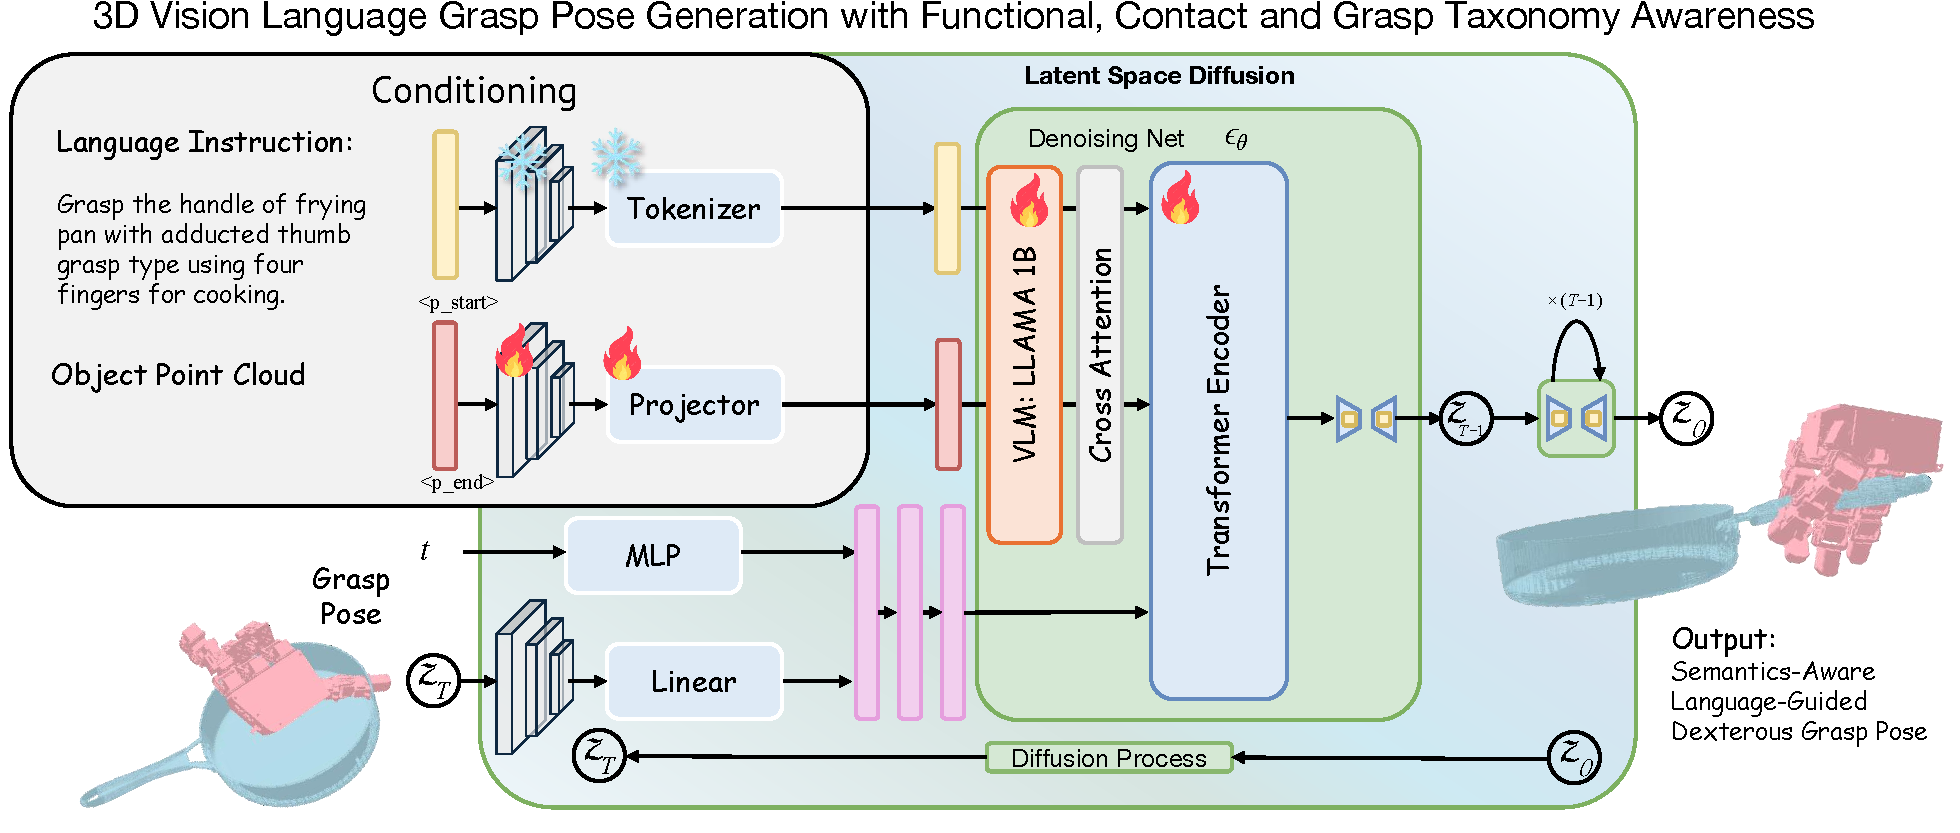
\includegraphics[width=1.0\linewidth]{pictures/fig04_network_structure.pdf}
  \caption{%
  % 
  OmniDexGraspNet: Vision Language Dexterous Hand Grasping Pose Generation Model. 
  The textual task description and the partial point cloud of the object are encoded into their respective latent features using a text encoder and a point cloud encoder. Simultaneously, the initial grasp pose is mapped into the latent space via a multilayer perceptron (MLP). These multimodal latent features are then fused and processed by a diffusion transformer encoder, which is trained to predict and remove noise in the grasp pose representation. This denoising process refines the grasp configuration to produce a physically plausible and task-relevant hand pose following language instruction. The input text instructions include key semantic elements such as the grasp affordance location, the intended grasp type, contact fonfiguration, and the high-level task objective.
  }
  \label{fig:network_structure}
\end{figure*}

\subsection{Vision Language Dexterous Hand Grasping Pose Action Generation Model}
\label{sec:3d_vision_language_dexterous_grasp_generation}

To enable effective perception and response to multi-dimensional semantic cues in dexterous grasping tasks, we propose a language-conditioned Vision-Language Grasping Generation (VLG) model that generates semantically aligned dexterous grasp poses $\mathbf{g} \in \mathbb{R}^d$ based on partial point cloud observations $P \in \mathbb{R}^{N \times 3}$ of the target object and language instruction $\mathcal{L}$, as shown in Fig.~\ref{fig:network_structure}. 
The model is capable of modeling and leveraging three key semantic dimensions: functional affordance, contact semantics, and grasp taxonomy, allowing it to produce grasp actions that are highly consistent with the task-specific semantic intent. 

The proposed network comprises the key components: 
Multimodal Conditioning Embedding 
and Grasp Pose Diffusion Generator. 
The input language instruction and point cloud are embedded into a shared semantic space via a Vision-Language Model (VLM):
\begin{equation}
\mathbf{c}=f_{\mathrm{VLM}}(\mathcal{L}, P)
\end{equation}
where $f_{\rm VLM}$ denotes a pretrained transformer-based model (e.g., LLaMA-1B) with cross-attention between the language and visual tokens. The output $c \in \mathbb{R}^{d_c}$ serves as a semantic condition for pose generation.

For aligning the vision-language model with point cloud encoder, the PointNet-based encoder, projector are trained following the training strategy from PointLLM~\cite{xu2025pointllm,xu2024pointllm}. During first training stage, the projector is trained using the multimodal alignment dataset with point clouds, images and natural language annotations~\cite{xu2025pointllm,xu2024pointllm}. The point cloud encoder extracts local geometric features $f_{\rm pcd}$ from partial object point clouds. The extracted features are passed through a projector that maps them into a shared multimodal embedding space to enable semantic alignment with language features from language tokenizer and encoder. 

The multimodal feature fusion module captures complex cross-modal relationships between visual geometry and linguistic semantics, enabling the model to understand what to grasp, how to grasp. 

Grasp pose diffusion transformer generator is introduced to generate semantically aligned grasp poses from semantic condition $c$. 
The grasp pose is represented as a latent variable $z_{\theta}$, generated by gradually denoising a Gaussian-initialized latent $\mathbf{z}_T \sim \mathcal{N}(0, I)$ through a conditional denoising network:

\begin{equation}
\mathbf{z}_0=\mathbf{z}_T-\sum_{t=1}^T \epsilon_\theta\left(\mathbf{z}_t, \mathbf{c}, t\right)
\end{equation}
where $\epsilon_\theta$ is the noise prediction network , conditioned on timestep $t$ and semantic features $\mathbf{c}$. 

The training pipeline consists of two main stages. After training projector for point cloud understanding, pose generator is trained with generated dexterous grasp dataset annotated with rich semantic labels based on proposed OmniDexDataGen and OmniDexReasoner. The OmniDexGraspNet is trained to generate high-quality grasp poses that are sensitive to multiple semantic conditions and adaptable to different language instructions.




